
\chapter{Optimization in Deep Learning}
% Authors: Yash Goel, Dae Young Kim, Marvin Singson Mananghaya
% Lecture date: 3/25/2019

Optimization is one of the important aspects of deep learning. In this chapter, we talk about the basics of parameter updating and the step size. Choosing a right step size can greatly reduce the training time. 

\section{Gradient Descent in 1-Dimension}
% Authors: Yash Goel, Dae Young Kim, Marvin Singson Mananghaya
% Lecture date: 3/25/2019
Gradient descent is one of the most popular optimization algorithms used in Deep Learning. We initialize weights randomly and update in the direction in which the value of the loss function $E$ descends the steepest in order to find the minimizer $w$. This direction can be found by taking the negative of the gradient. This process can be represented as:
$$ w = w - \eta\frac{\partial E}{\partial w}$$
where
\begin{eqnarray*}
w &=& \text{weight}\\
\eta &=& \text{learning rate}\\
\frac{\partial E}{\partial W} &=& \text{gradient of loss function with respect to the weight}
\end{eqnarray*}
The time until convergence by the algorithm is related to (but not limited to) the learning rate, as given by the formula. For instance, we consider a quadratic loss function to optimize. This function is convex and there exists a unique minimizer. The figure below represents the different scenarios for different step sizes.

\begin{figure}[t]
\centering
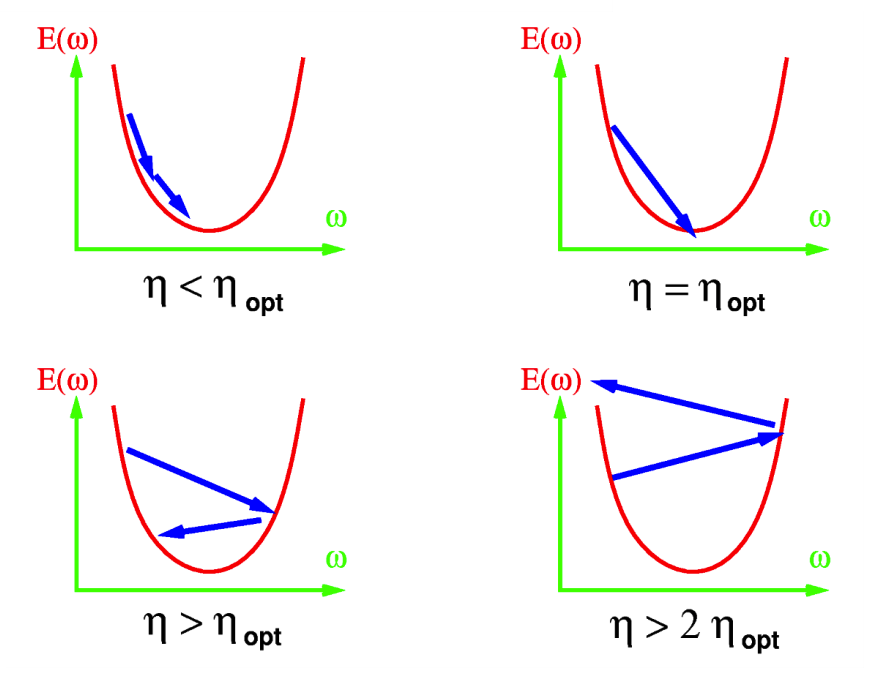
\includegraphics[width=100mm]{lectures/07-a/quadratic_function_to_optimise.png}
\caption{Various scenarios of tuning the learning rate.}
\end{figure}

\begin{itemize}
    \item For $\eta < \eta_{\textrm{opt}}$, the update takes small steps and longer time to the minimum.
    \item For $\eta=\eta_{\textrm{opt}}$, we have a convergence to the minimizer in one step.
    \item For $\eta > \eta_{\textrm{opt}}$, it bounces off the wall but still converges.
    \item For $\eta > 2 \eta_{\textrm{opt}}$, the update overshoots and we do not have convergence.
    
\end{itemize}

The question arises: "What's the optimal value for the learning rate $\eta$?" The optimal step size is given by computing the second derivative of the loss function.
$$ \eta_{opt} = (\frac{\partial^2 E}{\partial w^2})^{-1} $$
Therefore the weight update rule in this case is given by:
$$ w_{t+1} = w_t - (\frac{\partial^2 E}{\partial w_{t}^2})^{-1}\frac{\partial E}{\partial w_t}  $$
This is given by Newton's algorithm for optimization\footnote{https://en.wikipedia.org/wiki/Newton\%27s\_method\_in\_optimization}. Above example is for 1-Dimensional case, but it can also be generalized to multiple dimensions.


\section{Gradient Descent in n-Dimension}
% Authors: Yash Goel, Dae Young Kim, Marvin Singson Mananghaya
% Lecture date: 3/25/2019

In this section, we observe the gradient descent in multiple dimensions. Let $m$ be the dimension of input space and let us consider a single linear unit with $m$-dimensional inputs.
\begin{figure}[t]
\centering
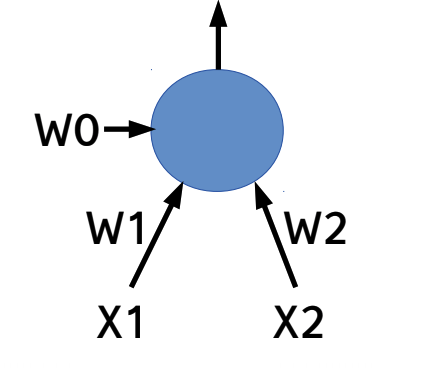
\includegraphics[width=50mm]{lectures/07-a/su.png}
\caption{A single linear unit with 2-dimensional input.}
\end{figure}
The quadratic loss function is given as follows: 
$$ E(\vect{W})= \frac{1}{P}\sum_{p=1}^P(Y_{p} - \vect{W}^{\top}\vect{X}_{p})^2$$
where $p$ refers to the index of the training data. We want to compute the gradient and the second derivative.

\begin{align*}
E(\vect{W}) &=\frac{1}{P}\sum_{p=1}^P(Y_{p} - \vect{W}^{\top}\vect{X}_{p})(Y_{p} - \vect{W}^{\top}\vect{X}_{p})\\
&= \frac{1}{P}\sum_{p=1}^P Y_{p}^2 - 2Y_{p}\vect{W}^{\top}\vect{X}_{p} + \vect{W}^{\top}\vect{X}_{p} \vect{X}_p^{\top}\vect{W}
\end{align*}
Taking the first and second derivative of $E(\vect{W})$ with respect to $\vect{W}$ gives us:
\begin{eqnarray*}
\frac{\partial E}{\partial \vect{W}} &=& -\frac{2}{P}\sum_{p}(Y_{p} - \vect{W}^{\top}\vect{X}_{p}) \vect{X}_{p}^\top\\
\frac{\partial^2 E}{\partial \vect{W}^2} &=&  \frac{2}{P}\sum_{p}\vect{X}_{p}\vect{X}_{p}^\top
\end{eqnarray*}
The second derivative turns out to be a covariance matrix of the input vectors, shaped as a symmetric matrix with $m \times m$ dimension. This matrix is also called as the Hessian Matrix, represented by $\matr{H}$. Therefore the update rule is now given by:
$$ \vect{W}_{t+1} = \vect{W}_t - \matr{H}^{-1}\frac{\partial E}{\partial \vect{W}_t} $$
The main takeaways are as follows. With the right learning rate, the gradient doesn't paddle left or right, and this also leads to the convergence to the global minimizer. Another thing to note is that when we tune the learning rate, it affects the speed of training but it is usually hard to find the optimal learning rate beforehand.

\section{Cost Function Appearance and Eigen-Decomposition}
% Authors: Yash Goel, Dae Young Kim, Marvin Singson Mananghaya
% Lecture date: 3/25/2019
From the previous section we observed the quadratic cost function.
\begin{align*}
E(\vect{W}) &= \frac{1}{P}\sum_{p=1}^P Y_{p}^2 - 2Y_{p}\vect{W}^{\top}\vect{X}_{p} + \vect{W}^{\top}\vect{X}_{p} \vect{X}_p^{\top}\vect{W}\\
\nabla E(\vect{W}) &= \frac{1}{P}\sum_{p=1}^P - 2Y_{p}\vect{X}_{p} + 2\vect{X}_{p} \vect{X}_p^{\top}\vect{W}\\
H = \nabla^2 E(\vect{W}) &= \frac{2}{P}\sum_{p=1}^P \vect{X}_{p} \vect{X}_p^{\top}
\end{align*}
The Taylor expansion of $E$ at the minimizer $\vect{W^*}$ is exact (no remainder term) and we get
$$E(\vect{W})  = E(\vect{W^*}) + (\vect{W}-\vect{W}^*)^{\top}\matr{H}(\vect{W}-\vect{W}^*)$$
The function $E$ is a quadratic function with respect to each input, and the Hessian matrix determines the curvature and orientation of each dimension. We study the diagonalization (eigen-decomposition) of H:
$$ \matr{H} = \matr{Q}\matr{\Lambda}\matr{Q}^\top$$
where $\matr{Q}$ is an orthogonal matrix (rotation into eigen-spaces) and $\matr{\Lambda}$ is a diagonal matrix (scaling in eigen-spaces). The gradient is orthogonal to the level sets (lines of equal cost) and the gradient is larger in a dimension where the curvature is larger. 

In practice, computing the Hessian is intractable. Even if it were, it might not be positive definite. Thus applying Newton's method to Deep learning might be hopeless, but there are other smart tricks: transforming the data and network in such a way that $\matr{H}$ has good properties.

\section{Examples with Input Characteristics Combinations}
% Authors: Yash Goel, Dae Young Kim, Marvin Singson Mananghaya
% Lecture date: 3/25/2019

\subsection{Case 1: Best Case}
% Authors: Yash Goel, Dae Young Kim, Marvin Singson Mananghaya
% Lecture date: 3/25/2019
Given $\mu_{x_{1},x_{2}} = 0$, $\sigma_{x_{1},x_{2}}^2 = 1$, and $x_1$ and $x_2$ are uncorrelated, this would result into a Hessian matrix being the identity matrix.
$$\matr{H} = \begin{bmatrix}
    1\;0\\
    0\;1\\
\end{bmatrix}$$ 
This is the best case as it means learning rate can be the same for both inputs $x_1$ and $x_2$, but what does it mean if the inputs have different characteristics?

\subsection{Case 2 : inputs have varying variances/standard deviations}
% Authors: Yash Goel, Dae Young Kim, Marvin Singson Mananghaya
% Lecture date: 3/25/2019
Given $\mu_{x_{1},x_{2}} = 0$, $\sigma_{x_{1}} = 1$, $\sigma_{x_{1}} = 2$, and $x_1$ and $x_2$ are uncorrelated, this would result into a Hessian with the following form:
$$\matr{H} = \begin{bmatrix}
    1\;0\\
    0\;4\\
\end{bmatrix}$$
This is problematic! Because the optimum learning rate for $x_1$ is $\frac{1}{4}$ of that of $x_2$, the maximum learning rate is limited to 4. Thus $x_1$ learns 4 times slower. The moral of the story is to make sure the input variable's variance is more or less the same or very close, commensurate. Things Professor LeCun mention in passing:
\begin{itemize}
    \item A lot of pre-processing is done by data loaders to ensure that variances normalize to one for standard datasets.
    \item For images, don't normalize all pixels individually. Normalize every channel by a single constant.
\end{itemize}
\subsection{Case 3: inputs resulting to different means}
% Authors: Yash Goel, Dae Young Kim, Marvin Singson Mananghaya
% Lecture date: 3/25/2019
Given $\mu_{x_{1},x_{2}} = 0$, $\sigma_{x_{1},x_{2}}^2 = 1$, and $x_1$ and $x_2$ are uncorrelated but $x_1$ and $x_2$ has 100 added to them, this would result into a Hessian with the following form:
$$\matr{H} = \begin{bmatrix}
    10001\;10000\\
    10000\;10001\\
\end{bmatrix}$$
This is terrible! This results to eigenvalues of 10,000 and 1 which result to a curvature that is 10,000 times larger in one direction compared to another.